% !TEX root = ../../../main.tex
% 来源：中学数学实验教材·第三册（高中数学）
% 章节：函数及其图象 / 一次函数（线性函数）
% 原始文件：4.tex，行 2225-2242
% 类型：tikz
% ---
    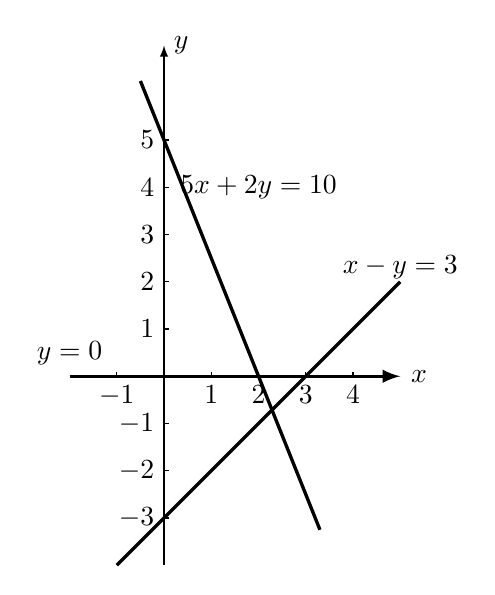
\begin{tikzpicture}[>=latex, scale=.6]
        \draw[->,very thick] (-2,0)node[above]{$y=0$}--(5,0)node[right]{$x$};
        \draw[->] (0,-4)--(0,7)node[right]{$y$};
        \foreach \x in {-1,1,2,...,4}
        {
            \draw (\x,0)node[below]{$\x$}--(\x,.1);
        }
    \foreach \y in {-3,-2,-1,1,2,...,5}
    {
        \draw (0,\y)node[left]{$\y$}--(.1,\y);
    }
    \draw [domain=-1:5, samples=10, very thick] plot(\x, {\x-3});
    \draw [domain=-.5:3.3, samples=10, very thick] plot(\x, {5-2.5*\x});
    
    \node at (2,4){$5x+2y=10$};
    \node at (5,2.3){$x-y=3$};
    
    \end{tikzpicture}
